\section{Transport Layer}

\subsection{UDP}

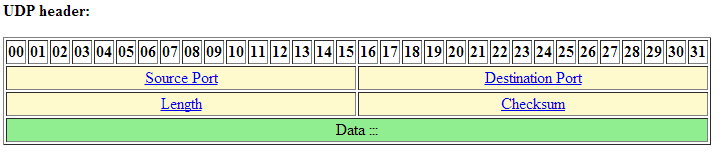
\includegraphics[scale=0.8]{media/UDPHeader.png}
Aufgepasst: Die Checksumme berücksichtigt auch den IP-Header und verletzt somit das Schichten Modell. \\
Das Längenfeld beinhaltet auch den UDP Header, ist also immer mindestens 8.
\\
\begin{align*}
Maximum Segment Size (MSS) = MTU - IPHeader - UDP Header = 1472\\
MTU = 1500Bytes\\
IPHeader = 20 Bytes
UDPHeader = 8Bytes
\end{align*}

\subsubsection{Analyse UDP Stream}

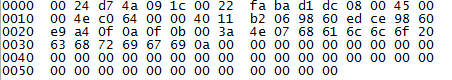
\includegraphics[scale=1.0]{media/UDPStream.png}

\textbf{MAC Header}\\
\begin{tabular}[h]{ll}
DST Address: & 00:24:D7:4A:09:1C\\
SRC Address: & 00:22:FA:BA:D1:DC\\
Ethertype: & 0x8000 (IP)\\
\end{tabular}


\textbf{IP Header}\\
\begin{tabular}[h]{ll}
Version \& IHL: & 0x45 (Version 4, IHL 5)\\
TOS: & 0x00\\
Total Length: & 0x004e (78 Bytes)\\
Identification: & 0xC064 (49252)\\
Flags \& Offset: & 0x0000\\
TTL: & 0x40 (128)\\
Protocol: & 0x11 (17/UDP)\\
Checksum: & 0xB206 \\
Src Address: & 0x98.0x60.0xED.0xCE (152.96.237.206)\\
Dst Address: 0x98.0x60.0xE9.0xA4 (152.96.233.164)\\
Option \& Padding: & -\\
\end{tabular}

\textbf{UDP Header}\\
\begin{tabular}[h]{ll}
Source Port: & 0x0F0A (3850)\\
Destination Port: & 0x0F0B (3851)\\
Length: 0x003A & (58 Bytes)\\
Checksum: & 0x4E07\\
Data: & hallo chrigi00000000.... (50 Bytes)
\end{tabular}


\subsection{TCP}

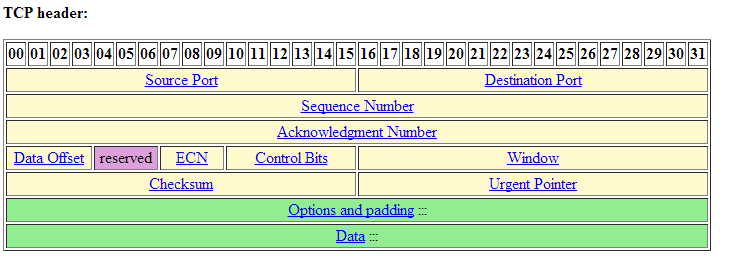
\includegraphics[scale=0.8]{media/TCPHeader.png}
Aufgepasst: Die Checksumme berücksichtigt auch den IP-Header und verletzt somit das Schichten Modell. \\
\begin{align*}
Maximum Segment Size (MSS) = MTU - IPHeader - TCP Header = 1460 Bytes\\
MTU = 1500Bytes\\
IPHeader = 20 Bytes\\
TCPHeader = min 20Bytes
\end{align*}
\subsubsection{Analyse TCP Stream}
\textbf{Cumulative ACK}\\
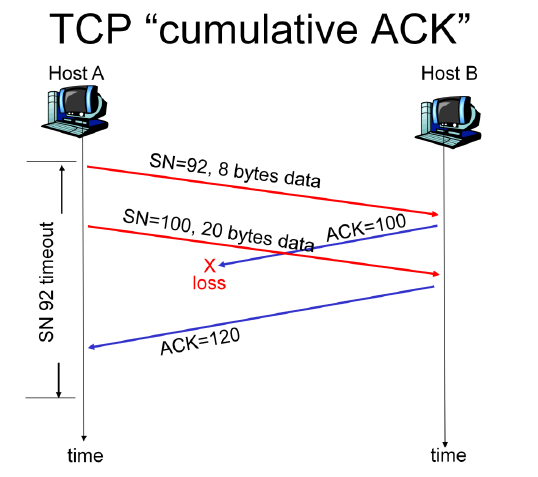
\includegraphics[scale=0.5]{media/cumulativeACK.png}\\
\textbf{Delayed ACK}\\
Im Prinzip wie Cumulative ACK. Die ACK Verluste sind aber absichtlich, d.h der Empfänger sendet nicht für jedes Paket ein ACK, sondern wartet auf eine der 2 Bedingugen:\\\\
1. TCPDelAckTicks: Ist nach Ablauf dieses Timers kein Paket mehr angekommen, sendet er ein kumulatives ACK. \\
2. TCPAckFrequency: Wurde für die festgelegte Anzahl Pakete kein ACK versendet, sendet er ein kumulatives ACK.\\

\subsubsection{TCP Flow Control}
\textbf{Window Size}\\
Mit dem Receive Window (RWin) gibt der Empfänger dem Sender an, wie viele Bytes der Sender noch schicken darf, ohne ein ACK erhalten zu haben. Receive Window ist die Receive Buffer Grösse des Empfängers.\\
Das Ziel ist es die Pipe zwischen Sender und Empfänger immer optimal zu füllen, sodass der Sender nicht auf ACK's warten muss. D.h Die Window Size sollte grösse sein als RTT * Bandbreite.\\
Schickt der Sender das erste Paket ab, dauert es eine RTT bis er ein ACK bekommt. Während dieser Zeit sollte der Sender aber fortlaufend weitere Pakete in die Pipe legen dürfen. Oder anders gesagt, die Anzahl Packete die der Sender während einer RTT in die Pipe legen kann ist das BDP (Bandwidth Delay Product). Die Window Size sollte optimalerweise mindestens so gross sein wie das BDP, da sonst auf ACK's gewartet werden muss.\\\\
$BDP=RTT \cdot Bandwidth$\\\\
Beispiel Kommunikation nach Thailand:\\
\begin{align*}
R_{WIN} = 50000 \frac{KBit}{s} \cdot 0.3s = 150000 KBits = 1875 KBytes
\end{align*}

\textbf{Maximum Distanzen}\\
Nachfolgend ein Beispiel für die Maximale Distanz (Füllung der Pipe) bei gegebener Window Size von 64KB und Geschwindigkeit von 1.5MBit/s
\begin{align*}
RTT = \frac{R_{WIN}}{R_{MAX}}\\
\end{align*}
\begin{align*}
\frac{64KB \cdot \frac{8Bit}{Byte} \cdot \frac{1024Bit}{KByte}}{\frac{1.5Mbit}{s}} = 0.35s
\end{align*}
\begin{align*}
Distance = v \cdot t =(\frac{2}{3} \cdot 300000 \frac{km}{s})\cdot 0.35s = 70000km
\end{align*}

\textbf{Duplicate Acknowledgement}\\
Der Empfänger sendet ein dup ACK (Acknowledgment, dass er bereits gesendet hat), d.h ein Paket vom Sender muss verloren gegangen sein. Nach 3 Dub ACK's (4 Identischen ACK's ohne weitere Pakete dazwischen, sendet der Sender das verlorengegangene Paket nochmals.


\textbf{Fast Retransmit}\\
Sobald ein Paket Out-of-Order empfangen wird, wird sofort ein dup ACK gesendet. Die Pakete die in der Zwischenzeit beim Empfänger ankommen werden jedoch behalten und nach einem allfälligen Retransmit kummulativ bestätigt.\\
Ein Dub ACK heisst, dass ein Paket Out-Of-Order ist, wobei 3 Pakete ein ziemlich sicheres indiz für ein Paketverlust ist.

\textbf{Selective ACK}\\
Die SACK Option muss beim Verbindungsaufbau im SYN aktiviert werden. 
Ein ACK mit SACK beinhaltet Block mit Daten, die bereits erfolgreich empfangen wurden. D.h die Daten unterhalb (ACK - beginn des Blocks) und oberhalb des Blocks müssen nochmals versandt werden. Die Blockstart bzw. end Oktett angaben werden mittels 32Bit Werten dargestellt. Ein Bock ist also 8 Bytes gross.
Die Maximalgrösse des TCP Headers ist 40 Bytes, demnach sind maximal 4 Blöcke (32Bytes) + Option Type / LEN (2Bytes) pro Paket möglich. Jedoch wird in diesem Zusammenhang auch noch die RTTM Option verwendet welche 10 + 2 Bytes benötigt verwendet. Somit bleibt nur noch für 3 Blöcke Platz.

\textbf{Congestion Window (cwnd) / Slow Start}\\
Das Congestion Window ist die Flusskontrolle auf Senderseite im Gegensatz zur Window Size welche die Flusskontrolle auf Empfängerseite darstellt. Die CWND Size wird jedoch nicht kommuniziert, sie stellt nur eine lokale Kontrollgrösse dar. Die CWND legt die Anzahl Segmente(MSS wird vom Empfänger mittgeteilt) fest, welche ohne ACK's gesendet werden können. Zu Beginn ist dieser Wert 1 (Slow Start) und wird nach jedem ACK erhöht. Schlussendlich gilt der kleinere Wert $min(cwnd,WindowSize)$ als MaxWin Size und bestimmt wieviele Segmente ohne ACK's höchstens gesendet werden dürfen.


\subsubsection{TCPTrace}
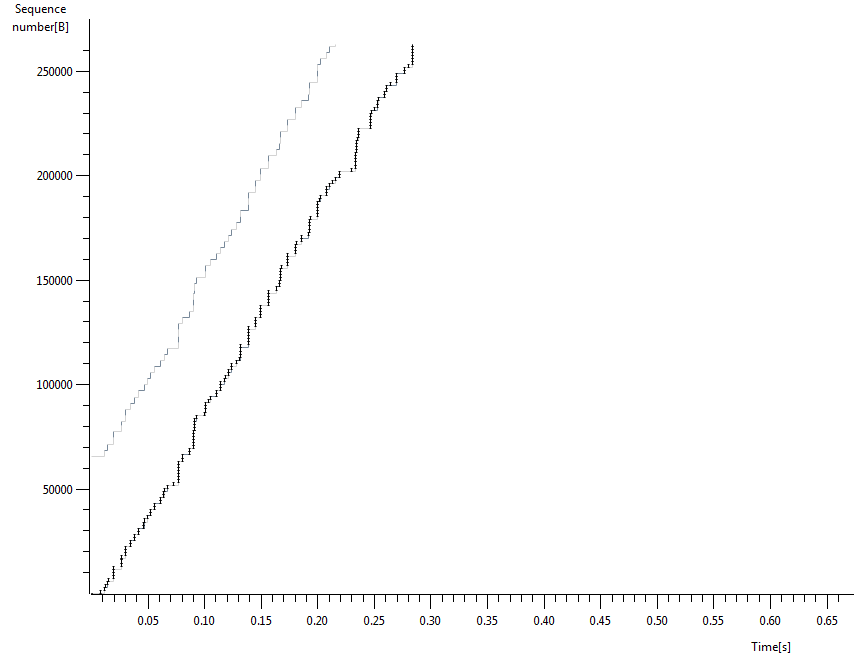
\includegraphics[scale=0.5]{media/tcptraceUpload.png}\\
Anhand der schnell ansteigenden Sequenznummern ist zu erkennen, dass es sich um einen Upload handelt.\\
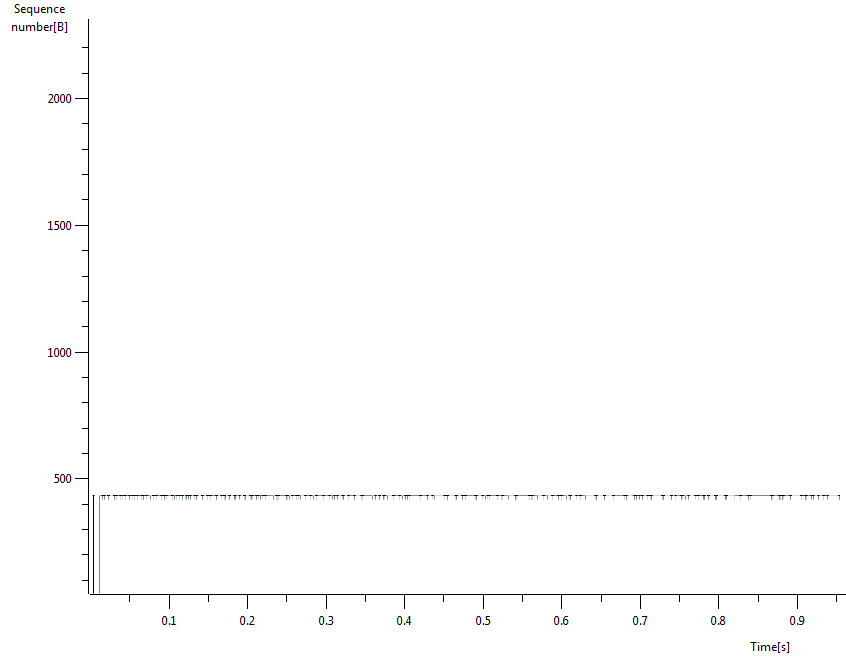
\includegraphics[scale=0.5]{media/tcptraceDownload.png}\\
Anhand der nur langsam erhöhenden Sequenznummer ist zu erkennen, dass nur sehr wenige Daten versendet werden und es sich somit um einen Download handelt.
